% Informe final - Práctica de investigación (Proyecto interno UNSAM)
% Compilar con XeLaTeX:  latexmk -xelatex informe_final.tex
\documentclass[11pt,a4paper]{article}

\usepackage{fontspec}
\usepackage{polyglossia}
\setdefaultlanguage{spanish}
\setmainfont{TeX Gyre Termes}
\setsansfont{TeX Gyre Heros}
\setmonofont{DejaVu Sans Mono}[Scale=0.82]

\usepackage[margin=2.5cm]{geometry}
\usepackage{graphicx}
\usepackage{xcolor}
\usepackage{booktabs}
\usepackage{tabularx}
\usepackage{array}
\usepackage{longtable}
\usepackage{enumitem}
\usepackage{caption}
\usepackage{listings}
\usepackage{fancyhdr}
\usepackage{titlesec}
\usepackage{csquotes}
\usepackage{amssymb}
\usepackage{tikz}
\usetikzlibrary{arrows.meta,positioning,fit,backgrounds,calc}
\usepackage[hidelinks]{hyperref}

\definecolor{pag12}{HTML}{C62828}
\definecolor{lanacion}{HTML}{1F5FAE}
\definecolor{gris}{HTML}{555555}
\definecolor{fondocod}{HTML}{F6F6F6}
\definecolor{pendiente}{HTML}{B00020}

% Marca visible para datos que la estudiante debe completar antes de entregar
\newcommand{\pendiente}[1]{\textcolor{pendiente}{\textbf{[#1]}}}

\captionsetup{font=small,labelfont=bf,labelsep=period}
\setlist{itemsep=2pt,topsep=4pt}
\setlength{\parskip}{4pt}
\setlength{\emergencystretch}{3em}

\titleformat{\section}{\large\bfseries\sffamily}{\thesection.}{0.6em}{}
\titleformat{\subsection}{\normalsize\bfseries\sffamily}{\thesubsection.}{0.6em}{}
\titleformat{\subsubsection}{\normalsize\itshape}{\thesubsubsection.}{0.6em}{}

\pagestyle{fancy}
\fancyhf{}
\fancyhead[L]{\small\color{gris}¿Qué es la Economía Popular? - Informe final}
\fancyhead[R]{\small\color{gris}M. S. Crespi}
\fancyfoot[C]{\small\thepage}
\renewcommand{\headrulewidth}{0.4pt}

\lstset{
  language=Python, basicstyle=\ttfamily\small, backgroundcolor=\color{fondocod},
  frame=single, rulecolor=\color{black!15}, breaklines=true, columns=fullflexible,
  keepspaces=true, showstringspaces=false, keywordstyle=\color{lanacion}\bfseries,
  commentstyle=\color{gris}\itshape, stringstyle=\color{pag12!80!black},
  numbers=left, numberstyle=\tiny\color{gris}, xleftmargin=1.6em, framexleftmargin=1.4em,
  captionpos=b, aboveskip=8pt, belowskip=6pt,
}
\renewcommand{\lstlistingname}{Código}
\renewcommand{\lstlistlistingname}{Índice de fragmentos de código}

\newcommand{\pdoce}{\textit{Página/12}}
\newcommand{\lanac}{\textit{La Nación}}
\newcommand{\EP}{economía popular}

\begin{document}

% =====================================================================
% CARÁTULA - Anexo III (se respeta la estructura del formulario)
% =====================================================================
\thispagestyle{empty}
{\small
\begin{center}
  
\includegraphics[height=1.3cm]{logo_unsam.png}\\[0.6em]
  {\small Licenciatura en Ciencia de Datos - UNSAM}\\[0.6em]
  {\Large\bfseries Anexo III}\\[0.3em]
  {\Large\bfseries Informe Final - Carátula}\\[0.4em]
  {\small\itshape Pasantías · Proyectos Profesionales Externos · Proyectos Internos · Producción Científica o Tesina}
\end{center}
\vspace{0.4em}

\noindent\textbf{Datos del estudiante}\\[-0.4em]
\rule{\linewidth}{0.4pt}\\
\textbf{Nombre y apellido:} María Sol Crespi

\vspace{0.35em}
\noindent\textbf{Tipo de actividad}\\[-0.4em]
\rule{\linewidth}{0.4pt}\\
\textit{Marcar con una X la opción correspondiente:}\\
$\square$\; Pasantía (propuesta desde la UNSAM)\\
$\square$\; Pasantía (externa)\\
$\square$\; Proyecto profesional externo a la UNSAM\\
$\boxtimes$\; Proyecto interno de la UNSAM\\
$\square$\; Producción científica o tesina

\vspace{0.4em}
\noindent\textbf{Título del proyecto o actividad:} ¿Qué es la Economía Popular? Una exploración a través de la prensa (2019--2023).

\vspace{0.35em}
\noindent\textbf{Director o responsable del proyecto}\\[-0.4em]
\rule{\linewidth}{0.4pt}\\
\textbf{Nombre y cargo:} Gabriela Delamata, Directora e investigadora; profesora en la EPyG.\\
\textbf{Institución / Unidad Académica:} Instituto de Investigaciones Políticas (IIP), Escuela de Política y Gobierno, UNSAM-CONICET.

\vspace{0.35em}
\noindent\textbf{Tutor}\\[-0.4em]
\rule{\linewidth}{0.4pt}\\
\textbf{Nombre y cargo:} Agustín Moro\\
\textbf{Institución / Unidad Académica:} Escuela de Ciencia y Tecnología, UNSaM

\vspace{0.35em}
\noindent\textbf{Créditos y optativa que solicita acreditar}\\[-0.4em]
\rule{\linewidth}{0.4pt}\\
\textit{El/la estudiante indica cuántos créditos solicita y a qué número de optativa los aplica, según su plan de acreditación.}\\
\textbf{Créditos que solicita acreditar:} 6\\
\textbf{Número de optativa a la que aplica:} 1\\
\textbf{Justificación breve de los créditos solicitados:} Se solicitan los 6 créditos previstos en el Plan de Trabajo (Anexo II) para proyectos internos, correspondientes a una dedicación de 96 horas entre agosto y noviembre de 2026. El trabajo cubrió la construcción completa de un corpus de prensa mediante extracción web, su procesamiento y codificación reproducible, la validación del método y la comunicación de resultados (ver secciones 2 y 3).

\vspace{0.35em}
\noindent\textbf{Materiales adjuntos}\\[-0.4em]
\rule{\linewidth}{0.4pt}\\
\textit{Marcar con una X lo que se acompaña:}\\
$\square$\; Documentación técnica\\
$\boxtimes$\; Código / notebooks / scripts\\
$\boxtimes$\; Modelos / visualizaciones / bases procesadas\\
$\square$\; Otro: \rule{6cm}{0.4pt}\\
$\square$\; No corresponde
}
\newpage
\setcounter{page}{1}

% =====================================================================
\begin{center}
  {\LARGE\bfseries ¿Qué es la Economía Popular?}\\[0.3em]
  {\large Una exploración a través de la prensa (2019--2023)}\\[0.8em]
  {\normalsize Informe final de práctica de investigación - Proyecto interno UNSAM}\\[0.2em]
  {\normalsize María Sol Crespi · Licenciatura en Ciencia de Datos, ECyT-UNSAM}\\[0.2em]
  {\small Dirección: Gabriela Delamata (IIP, EPyG, UNSAM-CONICET) · Tutor: Agustín Moro (ECyT, UNSAM)}\\[0.2em]
  {\small Noviembre de 2026}
\end{center}

\vspace{0.6em}
\noindent\fbox{\parbox{\dimexpr\linewidth-2\fboxsep-2\fboxrule}{\small
\textbf{Tipo de informe:} informe final.\quad
\textbf{Período:} 3 de agosto -- 13 de noviembre de 2026.\quad
\textbf{Dedicación prevista:} 96 horas.\quad
\textbf{Créditos solicitados:} 6.\quad
\textbf{Continuidad el próximo cuatrimestre:} No.}}

\vspace{0.8em}
\noindent\textbf{Resumen.} Este informe describe la práctica de investigación realizada en el marco de la convocatoria interdisciplinaria de datos e inteligencia artificial del CIAI, en articulación con el Instituto de Investigaciones Políticas de la Escuela de Política y Gobierno. Se construyó, mediante extracción web automatizada, un corpus de 1.245 notas de \lanac{} y \pdoce{} publicadas entre septiembre de 2019 y septiembre de 2023 que mencionan la expresión \enquote{\EP}. Sobre ese corpus se extrajeron 2.043 menciones y se codificaron, con el libro de códigos elaborado por el equipo de ciencias sociales, según quién enuncia el término (emisor) y en qué marco de referencia aparece. La codificación se realizó por dos vías que se compararon entre sí: un diccionario de patrones transparente y reproducible, y una lectura mención por mención, sobre las notas completas, asistida por un modelo de lenguaje. Los resultados muestran que el marco laboral es el predominante, que \pdoce{} lo asocia con mucha más frecuencia que \lanac{} (52\% frente a 34\% de las menciones de cada diario) y que \lanac{} asocia el término en mayor medida a la asistencia social, el conflicto y la figura del \enquote{piquetero}. La hipótesis de un desplazamiento temporal del marco laboral al asistencial y conflictivo encuentra un apoyo solo parcial: la diferencia más nítida se da entre diarios. El informe documenta también los ajustes respecto del plan original, las limitaciones del corpus y los aprendizajes de la práctica.

\tableofcontents
\newpage

% =====================================================================
\section{Objetivos originales planteados}
% =====================================================================

Se transcriben los objetivos tal como fueron previstos en el Plan de Trabajo (Anexo II).

\paragraph{Pregunta de investigación.} ¿Qué significó \enquote{\EP} en el discurso público argentino entre 2019 y 2023, quiénes hablaron en su nombre y dentro de qué marcos de referencia quedó inscripta?

\paragraph{Preguntas derivadas.}
\begin{itemize}
  \item ¿Se desplaza el término desde un marco laboral (sector, trabajo, cooperativa, paritaria) hacia uno asistencial (plan, subsidio, beneficiario) y contencioso (piquete, acampe, protesta)?
  \item ¿Qué emisores - estatales, sociales, periodísticos - aparecen asociados al término y cómo cambia esa composición a lo largo del período?
  \item ¿Difieren sistemáticamente los usos entre \lanac{} y \pdoce{}?
  \item ¿Los quiebres de la serie temporal coinciden con hitos políticos: creación de la UTEP en diciembre de 2019, ASPO e IFE en 2020, Potenciar Trabajo, cambios de gestión en Desarrollo Social, campaña de 2023?
\end{itemize}

\paragraph{Objetivo general.} Explorar, mediante el análisis computacional de un corpus de prensa nacional, el significado que la expresión \enquote{\EP} adquirió para un conjunto acotado de actores sociales y estatales de la Argentina entre 2019 y 2023, poniendo a prueba la hipótesis de que el término se volvió polisémico, disperso e incluso contrario a su significado original.

\paragraph{Objetivos específicos.}
\begin{enumerate}
  \item Construir una base de datos de notas periodísticas de \lanac{} y \pdoce{} publicadas entre el 01-09-2019 y el 30-09-2023 que mencionan el término \enquote{\EP}.
  \item Caracterizar el corpus mediante un análisis exploratorio: volumen de notas por mes y por diario, vocabulario predominante y evolución temporal de las menciones.
  \item Identificar, mediante reconocimiento de entidades nombradas, los emisores asociados a las menciones del término, distinguiendo emisores estatales, sociales y periodísticos.
  \item Calcular y visualizar las asociaciones entre emisores y el término mediante redes de co-ocurrencia, para el corpus general y por diario.
  \item Clasificar las menciones según su marco de referencia (sector, movimiento social, economía, política pública, política social, trabajo, trabajador, protesta, plan social) a partir de un diccionario de términos construido y validado con el equipo de investigación.
  \item Explorar, de manera complementaria, las asociaciones semánticas recurrentes del término mediante \textit{word embeddings} y el sentimiento asociado a sus menciones en cada diario.
  \item Producir visualizaciones comunicables en publicaciones académicas y en formato online, y documentar el proceso de modo reproducible.
\end{enumerate}

El Anexo II establecía que los objetivos 1 a 5 y 7 constituían el núcleo comprometido, y que el objetivo 6 era complementario y quedaba sujeto al avance de la construcción del corpus.

% =====================================================================
\section{Desarrollo del trabajo}
% =====================================================================

\subsection{Contexto y problema}

La categoría \enquote{\EP} fue acuñada por las organizaciones sociales argentinas a comienzos de la década de 2010 para nombrar un sujeto laboral preciso: trabajadoras y trabajadores sin patrón, excluidos del empleo formal, que generan su propio trabajo. Se trató de una identidad orientada al reconocimiento de derechos laborales, que encontró expresión legal en la personería social de la CTEP (2016) y en la Ley 27.345, que creó el registro de trabajadores de la economía popular, el salario social complementario y el Consejo de la Economía Popular. Entre 2019 y 2023 el término circuló en un escenario distinto: organizaciones integradas a la gestión estatal, la pandemia, la expansión de las transferencias de ingreso y la estigmatización pública de los llamados \enquote{planeros}. El proyecto del equipo dirigido por Gabriela Delamata busca observar ese desplazamiento en la prensa. Analíticamente se apoya en la noción de marcos interpretativos del estudio de los movimientos sociales (Benford y Snow, 2000).

\subsection{Rol de la estudiante y actividades realizadas}

La práctica se desarrolló en un equipo interdisciplinario. El equipo de ciencias sociales (Gabriela Delamata, Marina Farinetti, Martina Tomada y Daniela Porfirio) definió la pregunta, la hipótesis y el libro de códigos. Mi rol fue el de ciencia de datos: diseñar e implementar la recolección del corpus, el procesamiento de los textos, la codificación automática de las menciones, su validación, el análisis de los resultados y su comunicación. La orientación técnica sobre extracción web estuvo a cargo del CIAI.

\begin{table}[h]
\centering\small
\caption{Actividades realizadas por período.}
\label{tab:cronograma}
\begin{tabularx}{\linewidth}{>{\raggedright}p{2.6cm} X >{\raggedright\arraybackslash}p{4.2cm}}
\toprule
\textbf{Período} & \textbf{Actividades} & \textbf{Productos} \\
\midrule
Agosto & Lectura del marco conceptual; elaboración del Plan de Trabajo; reunión de orientación técnica sobre extracción web con el CIAI (31/08), en la que se definió la automatización de navegador. & Anexo II; estrategia de extracción. \\
Septiembre & Recolector de \pdoce{} (API interna del buscador); recolección de enlaces de \lanac{} y recuperación de textos vía Wayback Machine; análisis exploratorio preliminar. & Corpus de \pdoce{}; corpus parcial de \lanac{}; informe de avance al equipo (29/09). \\
Octubre & Recolección de \lanac{} con la suscripción institucional; extracción de menciones; codificación por diccionario con el libro de códigos; validación por lectura de una muestra de 50 notas y lectura completa asistida por IA. & Corpus de 1.245 notas; base de 2.043 menciones codificadas; tablas emisor $\times$ marco; comparación de métodos. \\
Noviembre & Corrección del diccionario (marco \enquote{trabajo}); revisión de casos mal atribuidos; presentación en las Primeras Jornadas Interdisciplinarias de Ciencia de Datos e IA (04/11); informe final. & Script corregido; presentación; este informe. \\
\bottomrule
\end{tabularx}
\end{table}

\subsection{Herramientas}

\begin{itemize}
  \item \textbf{Python} como lenguaje principal; \textbf{Playwright} para la automatización de navegador; \textbf{pandas} y \textbf{openpyxl} para el manejo de datos; \textbf{re} (expresiones regulares) para la detección de menciones y la codificación; \textbf{matplotlib} para las visualizaciones.
  \item \textbf{Google Colab} y \textbf{Google Drive} como entorno de ejecución y almacenamiento, con puntos de control (\textit{checkpoints}) para retomar procesos largos.
  \item \textbf{DevTools} del navegador para inspeccionar el tráfico de red de los sitios y encontrar las fuentes de datos internas.
  \item \textbf{Claude} (Anthropic), un asistente de inteligencia artificial, usado para escribir y depurar código y para la lectura completa del corpus descripta en la sección~\ref{sec:lectura-ia}. Su uso se consigna aquí tal como lo establece el Plan de Trabajo.
\end{itemize}

\subsection{Arquitectura de la solución}

El procesamiento se organizó como una cadena de etapas independientes. Cada etapa lee la salida de la anterior desde una carpeta común en Google Drive y guarda la suya, de modo que cualquier etapa puede volver a ejecutarse sin repetir las anteriores (Figura~\ref{fig:pipeline}).

\begin{figure}[h]
\centering
\begin{tikzpicture}[
  font=\small\sffamily,
  etapa/.style={draw=black!70, rounded corners=3pt, fill=black!4, align=center, minimum height=1.3cm, text width=2.7cm, inner sep=4pt},
  archivo/.style={align=center, font=\scriptsize\ttfamily, text=gris},
  flecha/.style={-{Stealth[length=2.4mm]}, thick, black!70}]
  \node[etapa] (fuentes) at (0,0) {\textbf{Fuentes}\\Página/12: API\\La Nación: archivo web\\+ suscripción};
  \node[etapa] (corpus) at (3.7,0) {\textbf{1. Corpus}\\texto completo\\(Fusion/Arc XP)};
  \node[etapa] (menc) at (7.4,0) {\textbf{2. Menciones}\\regex + ventana\\de 300 caracteres};
  \node[etapa] (cod) at (11.1,0) {\textbf{3. Diccionario}\\emisor $\times$ marco\\(libro de códigos)};
  \node[etapa] (ia) at (3.7,-2.6) {\textbf{3'. Lectura completa}\\asistida por IA\\(mismas menciones)};
  \node[etapa] (val) at (7.4,-2.6) {\textbf{4. Validación}\\muestra de 50 notas;\\comparación de métodos};
  \node[etapa] (res) at (11.1,-2.6) {\textbf{5. Resultados}\\tablas, gráficos,\\presentación};
  \draw[flecha] (fuentes) -- (corpus);
  \draw[flecha] (corpus) -- (menc);
  \draw[flecha] (menc) -- (cod);
  \draw[flecha] (corpus) -- (ia);
  \draw[flecha] (ia) -- (val);
  \draw[flecha] (cod.south) -- ++(0,-0.45) -| (val.north);
  \draw[flecha] (val) -- (res);
  \draw[flecha, dashed] (val.south) -- ++(0,-0.45) -| node[pos=0.25, below, font=\scriptsize] {corrección del diccionario} (cod.south east);
\end{tikzpicture}
\caption{Arquitectura del procesamiento. Cada etapa guarda su salida en Drive y puede reejecutarse por separado. La lectura asistida por IA (3') trabaja sobre las mismas 2.043 menciones que la codificación por diccionario y se usa para validarla.}
\label{fig:pipeline}
\end{figure}

\subsection{Construcción del corpus}

El objetivo era reunir todas las notas de ambos diarios publicadas entre el 1 de septiembre de 2019 y el 30 de septiembre de 2023 que contuvieran la expresión \enquote{\EP}. Para cada nota se registraron medio, título, fecha, autor, sección, volanta o bajada, texto completo y enlace. Se eligió la automatización de navegador (Playwright) porque los buscadores de ambos sitios cargan sus resultados de forma dinámica con JavaScript, lo que impide la descarga directa del HTML.

\subsubsection{Página/12: la API interna del buscador}

Al inspeccionar con las DevTools el tráfico que genera el buscador del sitio se encontró la API interna que lo alimenta (un servicio Solr sobre la plataforma Arc XP). Consultarla directamente resultó más rápido y más preciso que recorrer la página con desplazamientos. El Código~\ref{cod:p12} muestra cómo se arma la consulta.

\begin{lstlisting}[caption={Armado de la consulta a la API de búsqueda de \pdoce.}, label=cod:p12]
PAGINA12_API_URL = "https://www.pagina12.com.ar/pf/api/v3/content/fetch/p12-solr-search"
PAGINA12_TAMANO_PAGINA = 100

def _armar_url_busqueda_pagina12(query, offset):
    query_obj = {
        "author": "", "endDate": "", "startDate": "", "section": "",
        "offset": offset,
        "page": offset // PAGINA12_TAMANO_PAGINA,
        "q": f'"{query}"',  # comillas = frase exacta
        "size": PAGINA12_TAMANO_PAGINA,
    }
    qs = quote_plus(json.dumps(query_obj, ensure_ascii=False, separators=(",", ":")))
    return f"{PAGINA12_API_URL}?query={qs}&d=132&mxId=00000000&_website=pagina12"
\end{lstlisting}

Tres hallazgos de esta etapa se obtuvieron probando un cambio por vez:
\begin{itemize}
  \item \textbf{Las comillas son necesarias.} Sin ellas la API devolvía 82.690 resultados (notas con \enquote{economía} o con \enquote{popular}); con la frase entre comillas, 2.330.
  \item \textbf{El filtro de fecha se aplica después.} Los parámetros \texttt{startDate} y \texttt{endDate} hacían fallar el pedido (error 404), por lo que se descargan los resultados y se filtran por fecha en Python.
  \item \textbf{El pedido debe salir desde el propio sitio.} La API solo responde a pedidos originados en una página de \pdoce. Por eso el script abre primero la portada y lanza el pedido desde allí con \texttt{page.evaluate(fetch(...))}.
\end{itemize}

\subsubsection{Extracción del texto completo}

Ambos diarios publican sobre el mismo sistema de gestión de contenidos (Fusion/Arc XP), que deja los datos completos de cada nota en una variable de JavaScript de la página. Leer esa estructura resultó más estable que depender de clases CSS, que cambian con cada rediseño, y permitió usar el mismo extractor para los dos medios (Código~\ref{cod:fusion}).

\begin{lstlisting}[caption={Lectura de los datos de una nota desde la estructura de Fusion/Arc XP.}, label=cod:fusion]
datos = await page.evaluate("() => window.Fusion && window.Fusion.globalContent")
titulo = (datos.get("headlines") or {}).get("basic")
fecha = datos.get("display_date")
seccion = ((datos.get("taxonomy") or {}).get("primary_section") or {}).get("name")
parrafos = [e.get("content") for e in datos.get("content_elements", [])
            if e.get("type") == "text"]
texto_completo = _limpiar_html("\n".join(parrafos))
\end{lstlisting}

\subsubsection{La Nación: del archivo web a la suscripción institucional}

\lanac{} fue la parte más costosa del proyecto. Su buscador no expone una API accesible y su muro de pago medido bloquea la lectura después de unas pocas notas. El trabajo pasó por dos etapas:
\begin{enumerate}
  \item \textbf{Archivo web.} Los enlaces se recolectaron recorriendo el buscador del sitio y el texto se recuperó de copias archivadas en Wayback Machine (archive.org), consultando su API CDX para cada enlace. La recolección por desplazamiento arrastraba unos 13.000 enlaces, la mayoría de notas relacionadas o recomendadas; en lugar de afinar selectores frágiles, ese ruido se descartó al final, conservando solo las notas cuyo texto contiene el término.
  \item \textbf{Suscripción institucional.} La directora del proyecto habilitó una suscripción. Como Google no permite iniciar sesión desde ventanas controladas por scripts, el inicio de sesión se hizo manualmente en un navegador común y Playwright se conectó luego a esa sesión para conservarla (Código~\ref{cod:sesion}). Esta etapa solo procesó los enlaces que el archivo web no había podido resolver.
\end{enumerate}

\begin{lstlisting}[caption={Captura de una sesión iniciada manualmente, para reutilizarla en la recolección.}, label=cod:sesion]
async def main():
    async with async_playwright() as p:
        browser = await p.chromium.connect_over_cdp("http://localhost:9222")
        context = browser.contexts[0]
        await context.storage_state(path=str(ARCHIVO_SESION))
\end{lstlisting}

En ningún momento se implementaron mecanismos para eludir el muro de pago: el texto de \lanac{} proviene de copias públicas archivadas o de la suscripción autorizada. Se trabajó con demoras entre pedidos y el archivo de sesión se trató como una credencial, sin versionarlo ni compartirlo.

\subsubsection{Corpus resultante}

El corpus final reúne \textbf{1.245 notas}: 645 de \lanac{} y 600 de \pdoce{}. De ellas, 1.215 tienen texto completo; las 30 restantes son de \pdoce{} y quedaron sin texto. La Figura~\ref{fig:trimestre} muestra la distribución temporal. El volumen crece en 2022, año con mayor cantidad de notas (432), y el trimestre de mayor actividad es el tercero de 2022 (145 notas), período de alta conflictividad en torno a los programas sociales.

\begin{figure}[h]
\centering
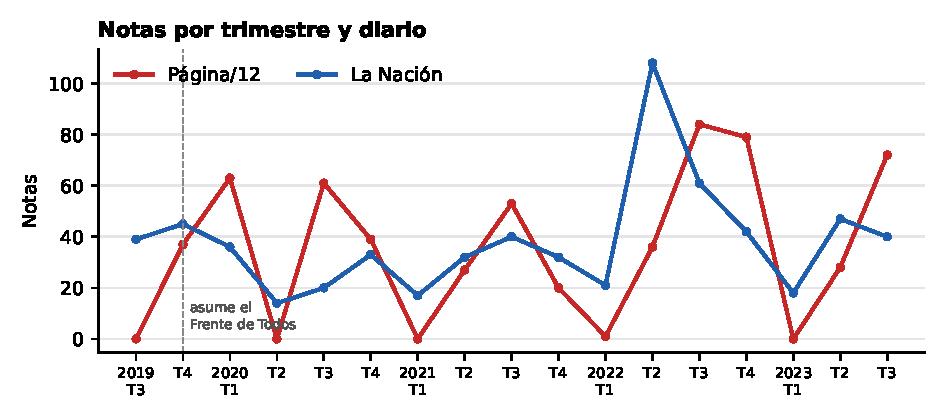
\includegraphics[width=\linewidth]{fig/fig_notas_trimestre.pdf}
\caption{Notas del corpus por trimestre y diario (\pdoce{} en rojo, \lanac{} en azul). Los trimestres sin notas de \pdoce{} reflejan una limitación de la recolección, discutida en la sección~\ref{sec:limitaciones}.}
\label{fig:trimestre}
\end{figure}

\subsection{Extracción de menciones}

La unidad de análisis es la \emph{mención}: cada aparición de \enquote{\EP} en el cuerpo de la nota. Una expresión regular tolerante a tildes, mayúsculas y plurales detecta cada aparición y recorta un fragmento de contexto de 300 caracteres antes y después. El mismo script registra un verbo de atribución cercano (\enquote{afirmó}, \enquote{sostuvo}, \enquote{señaló}, etc.) y un nombre propio candidato, como pistas para la lectura (Código~\ref{cod:menciones}). Se obtuvieron \textbf{2.043 menciones} en 1.204 notas: 1.059 en \pdoce{} y 984 en \lanac.

\begin{lstlisting}[caption={Detección de menciones y recorte del contexto (\texttt{extraer\_fragmentos.py}).}, label=cod:menciones]
PATRON_MENCION = re.compile(r"econom[ií]as?\s+popular(?:es)?", re.IGNORECASE)
VENTANA_CHARS = 300

def _ventana(texto, inicio, fin):
    desde = max(0, inicio - VENTANA_CHARS)
    hasta = min(len(texto), fin + VENTANA_CHARS)
    return texto[desde:hasta].replace("\n", " ").strip(), desde

for m in PATRON_MENCION.finditer(texto):
    fragmento, desde = _ventana(texto, m.start(), m.end())
    actor, verbo = _actor_candidato(fragmento, m.start() - desde)
\end{lstlisting}

\subsection{Codificación de emisores y marcos}

\subsubsection{Libro de códigos}

El libro de códigos, elaborado por el equipo de ciencias sociales, define dos dimensiones por mención. La primera es el \textbf{emisor}, es decir, quién enuncia o a quién se atribuye lo que se dice sobre la \EP{}, clasificado en cinco tipos con subtipos (Tabla~\ref{tab:codebook}). La segunda es el \textbf{marco de referencia}, es decir, con qué se asocia la \EP{} en esa mención, con 16 categorías: organizaciones de la economía popular, movimientos sociales, sector, políticas sociales y laborales, trabajadores informales, pobres, humildes, piqueteros, derechos, IFE, Potenciar Trabajo, trabajo/trabajadores, asistencia social, informalidad/precarización, conflicto/orden público e integración económica/desarrollo productivo. Una mención puede tener más de un emisor y más de un marco.

\begin{table}[h]
\centering\small
\caption{Tipos de emisor del libro de códigos.}
\label{tab:codebook}
\begin{tabularx}{\linewidth}{>{\raggedright}p{4.3cm} X}
\toprule
\textbf{Tipo} & \textbf{Subtipos y ejemplos} \\
\midrule
Estatal & Presidente; área social (Desarrollo Social, INAES); área económica y laboral; gobiernos subnacionales; otros poderes del Estado \\
Organizaciones y movimientos & UTEP y sus organizaciones (Movimiento Evita, Barrios de Pie, MTE, CCC); Patria Grande; izquierda y no alineadas; sindicatos tradicionales \\
Dirigentes sociales & Juan Grabois, Emilio Pérsico, Esteban \enquote{Gringo} Castro, entre otros \\
Sector privado & Cámaras y entidades empresarias \\
Otros, medios y academia & Voz del propio diario, notas de opinión, especialistas, Iglesia \\
\bottomrule
\end{tabularx}
\end{table}

\subsubsection{Codificación por diccionario}

La primera vía de codificación es un diccionario de patrones: para cada emisor y cada marco se definió una lista de expresiones regulares que se buscan en el fragmento. Para los emisores estatales se incluyeron la persona y el cargo, porque los cargos cambiaron de titular durante el período (Código~\ref{cod:emisores}). Se eligió este método porque es transparente y cualquier integrante del equipo puede revisar y corregir los patrones.

\begin{lstlisting}[caption={Fragmento del diccionario de emisores (\texttt{analisis\_emisores\_marcos.py}).}, label=cod:emisores]
EMISORES = {
    "Presidente de la Nación": (T1, S1A, N(
        "Alberto Fernández", "Mauricio Macri", "Presidencia de la Nación",
        r"re:\bel\s+presidente\b(?!\s+(?:de|del)\s+(?!la\s+naci[oó]n))",
        "Gobierno nacional", "Casa Rosada",
    )),
    "Ministerio de Desarrollo Social / Economía Social": (T1, S1B, N(
        "Daniel Arroyo", "Arroyo", "Juan Zabaleta",
        "Ministerio de Desarrollo Social", "ministro de Desarrollo Social",
        "Secretaría de Economía Social", "Alexandre Roig", "INAES",
    )),
    "UTEP / CTEP": (T2, S2A, N("UTEP", "CTEP", ...)),
    "Juan Grabois": (T3, "Dirigente social", N("Juan Grabois", "Grabois")),
    # ...
}
\end{lstlisting}

La función auxiliar \texttt{tol} convierte cada frase en una expresión regular tolerante a tildes y a espacios múltiples, de modo que \enquote{Persico} también reconoce \enquote{Pérsico}. El nombre completo de una organización que contiene el término (\enquote{Unión de Trabajadores de la Economía Popular}) no cuenta por sí solo como emisor: se elimina del fragmento antes de buscar.

\paragraph{Corrección del marco \enquote{trabajo}.} La validación (sección~\ref{sec:validacion}) mostró que el marco \enquote{trabajo/trabajadores} se activaba con el propio nombre de la UTEP, la CTEP y el RENATEP, que incluyen la palabra \enquote{trabajadores}. El script ya excluía esos nombres para los emisores, pero no para los marcos. Se corrigió la función \texttt{detectar\_marcos} para buscar ese marco sobre el fragmento sin esos nombres (Código~\ref{cod:marcos}). Con el script original sobre los mismos datos el marco aparecía en 1.366 menciones; con la corrección, en \textbf{881}. Los demás marcos no cambian; el de integración económica conserva a propósito el nombre del RENATEP como indicador.

\begin{lstlisting}[caption={Corrección de la detección de marcos.}, label=cod:marcos]
MARCOS_SIN_NOMBRES = {"Trabajo / trabajadores"}

def detectar_marcos(fragmento):
    if not isinstance(fragmento, str):
        return []
    limpio = PATRON_NOMBRE_CON_TERMINO.sub(" ", fragmento)
    return [n for n, p in MARCOS_COMPILADOS.items()
            if p.search(limpio if n in MARCOS_SIN_NOMBRES else fragmento)]
\end{lstlisting}

\subsubsection{Lectura completa asistida por IA}
\label{sec:lectura-ia}

La segunda vía se usó para validar la primera. Las 2.043 menciones se leyeron una por una con un asistente de inteligencia artificial (Claude, de Anthropic), siguiendo el mismo libro de códigos. Las notas se dividieron en 45 lotes, con todas las menciones de una misma nota en el mismo lote, y cada lote fue codificado por un agente lector distinto con las mismas instrucciones. Cada aparición del término estaba marcada en el texto de la nota, y los lectores no veían el resultado del diccionario. Las instrucciones incluían criterios explícitos: codificar como emisor a quien pronuncia el término y no a quien es mencionado; asignar un marco solo si el pasaje relaciona efectivamente la \EP{} con él; marcar las menciones que son solo parte de un nombre propio; y registrar los casos ambiguos en una columna de dudas. Esta vía tiene dos ventajas sobre el diccionario: lee la nota entera, por lo que reconoce a quien habla aunque se lo presente varios párrafos antes, y reconoce la voz del propio diario, que no tiene un nombre que buscar. Su principal riesgo es la variación de criterio entre lotes. Antes de procesar todo se hizo una prueba con 30 menciones, y algunas reglas se aclararon durante la lectura; el 47\% de las menciones tiene una duda registrada.

Una primera lectura, hecha por párrafo, había totalizado 1.961 menciones e incluía título y bajada, por lo que no podía compararse fila por fila con el diccionario. La idea de reunir ambas lecturas en una sola base surgió en las Primeras Jornadas Interdisciplinarias de Ciencia de Datos e Inteligencia Artificial (4 de noviembre de 2026), donde se presentaron los primeros resultados. La lectura actual la reemplaza y se hizo sobre las mismas 2.043 filas: los totales coinciden y la comparación es de uno a uno. La lectura se toma como referencia para medir el acuerdo, pero no es una verdad absoluta, porque todavía falta validarla con el equipo.

\subsection{Resultados}

Salvo indicación en contrario, las cifras de esta sección provienen de la codificación por diccionario corregida, que es reproducible a partir del código entregado. Siguiendo el criterio acordado con la dirección, todos los resultados se presentan separados por diario.

\subsubsection{Marcos de referencia}

El marco \enquote{trabajo/trabajadores} es el más frecuente en los dos diarios, pero con un peso muy distinto: aparece en el 52\% de las menciones de \pdoce{} y en el 34\% de las de \lanac{} (Figura~\ref{fig:marcos}). \lanac{} asocia la \EP{} en mayor proporción a la asistencia social (24\% frente a 20\%), al conflicto y el orden público (17\% frente a 10\%), al programa Potenciar Trabajo (12\% frente a 5\%) y a la figura del piquetero (5,1\% frente a 0,7\%). \pdoce{}, en cambio, la presenta más como un \enquote{sector} (23\% frente a 16\%) y en relación con los derechos (8,6\% frente a 4,5\%).

\begin{figure}[h]
\centering
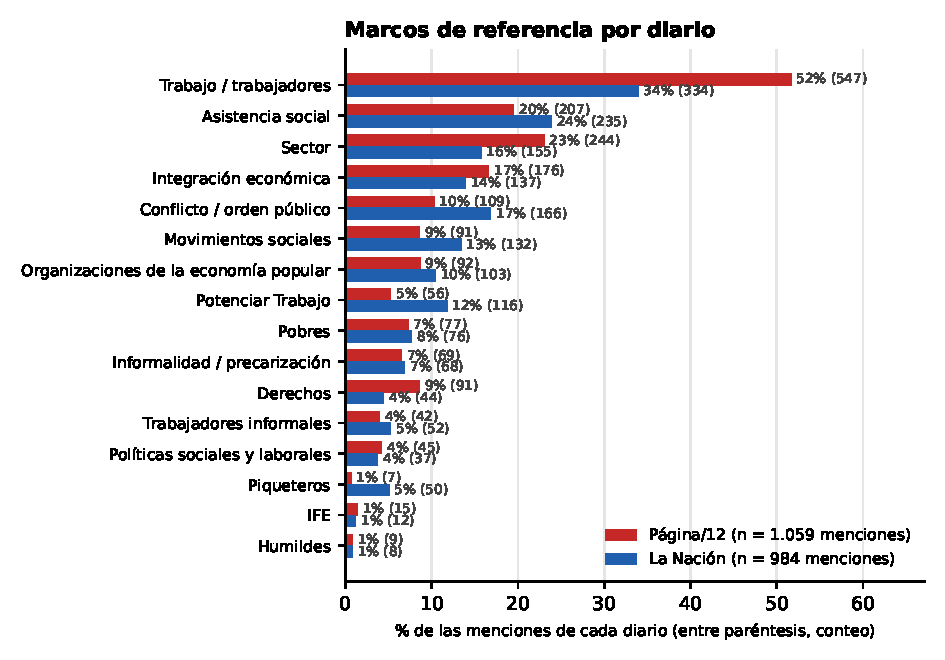
\includegraphics[width=\linewidth]{fig/fig_marcos_diario.pdf}
\caption{Marcos de referencia por diario: porcentaje de las menciones de cada diario en que aparece cada marco. Una mención puede tener más de un marco.}
\label{fig:marcos}
\end{figure}

\subsubsection{Emisores}

En ambos diarios las organizaciones y movimientos son el tipo de emisor más frecuente, seguidas por el Estado (Figura~\ref{fig:emisores}). La diferencia más marcada está en los dirigentes sociales, que aparecen en el 32\% de las menciones de \lanac{} y en el 9\% de las de \pdoce. Entre los emisores individuales, los más frecuentes son la UTEP/CTEP (628 menciones), la Presidencia de la Nación (233), otras organizaciones de la UTEP (222), Juan Grabois (213) y el Movimiento Evita (192). Grabois tiene un peso particular en \lanac{} (170 menciones frente a 43). El sector privado es marginal (4\% del total). El 36\% de las menciones no tiene un emisor detectado por el diccionario; en \pdoce{} la proporción llega al 45\%.

\begin{figure}[h]
\centering
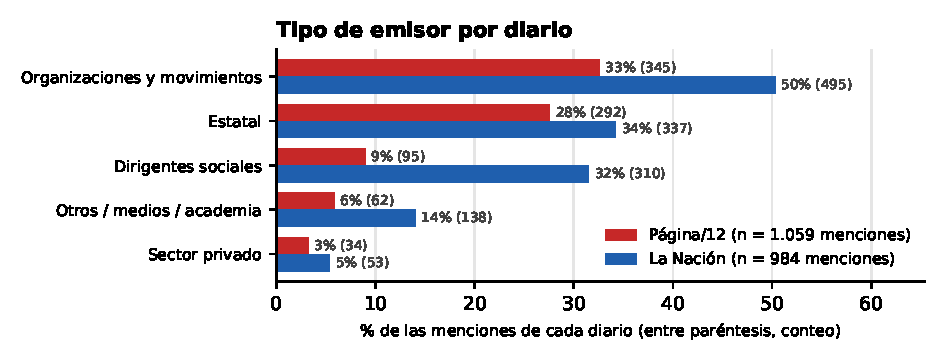
\includegraphics[width=\linewidth]{fig/fig_emisores_diario.pdf}
\caption{Tipos de emisor por diario: porcentaje de las menciones de cada diario.}
\label{fig:emisores}
\end{figure}

\subsubsection{Evolución temporal y la hipótesis}

La Figura~\ref{fig:anio} sigue por año los tres marcos que la hipótesis pone en juego. En \pdoce{} el marco laboral se mantiene estable, en torno al 50\%, y desciende en 2023 (42\%). En \lanac{} el marco laboral oscila entre 26\% y 44\%. La asistencia social muestra un pico claro en \lanac{} en 2022 (37\% de sus menciones), asociado a la discusión sobre los programas sociales, que no se sostiene en 2023. El conflicto es sistemáticamente más alto en \lanac{} y crece en los dos diarios en 2022.

\begin{figure}[h]
\centering
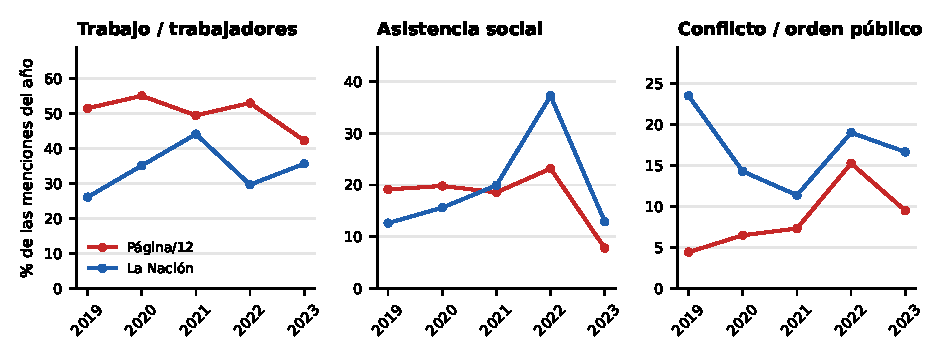
\includegraphics[width=\linewidth]{fig/fig_marcos_anio.pdf}
\caption{Porcentaje de las menciones de cada año y diario en que aparecen los marcos trabajo, asistencia social y conflicto. 2019 (septiembre a diciembre) y 2023 (enero a septiembre) son años parciales.}
\label{fig:anio}
\end{figure}

En síntesis, la hipótesis de un desplazamiento del marco laboral hacia uno asistencial y contencioso durante el gobierno del Frente de Todos encuentra \textbf{apoyo parcial}. Hay un aumento del marco asistencial y conflictivo en 2022, concentrado en \lanac, pero no un desplazamiento sostenido del marco laboral, que sigue siendo central en \pdoce{} durante todo el período. La diferencia más clara es entre diarios: cada uno inscribe el término en marcos distintos. Estas comparaciones deben leerse junto con las limitaciones del corpus de \pdoce{} (sección~\ref{sec:limitaciones}).

\subsubsection{Comparación entre métodos}

La Tabla~\ref{tab:metodos} compara los conteos de las dos vías de codificación, sobre las mismas 2.043 menciones. Los totales son parecidos en el marco laboral una vez corregido el diccionario (881 frente a 788) y en el de conflicto (275 frente a 242). Las diferencias más grandes están en la voz del propio medio, que el diccionario casi no detecta (200 frente a 1.313); en las organizaciones y movimientos, que el diccionario registra cuando aparecen cerca del término aunque no sean quienes hablan (840 frente a 129); y en el marco de políticas sociales y laborales (82 frente a 775), que el diccionario busca por frases exactas poco frecuentes en la prensa. Que dos totales se parezcan no implica que coincidan en las mismas menciones: el acuerdo fila por fila se analiza en la sección~\ref{sec:validacion}.

\begin{table}[h]
\centering\small
\caption{Menciones según cada vía de codificación, sobre las mismas 2.043 menciones.}
\label{tab:metodos}
\begin{tabular}{lrr}
\toprule
 & \textbf{Diccionario} & \textbf{Lectura con IA} \\
\midrule
\multicolumn{3}{l}{\textit{Marcos}} \\
\quad Trabajo / trabajadores (sin nombre de la UTEP) & 881 & 788 \\
\quad Políticas sociales y laborales & 82 & 775 \\
\quad Integración económica & 313 & 407 \\
\quad Conflicto / orden público & 275 & 242 \\
\quad Solo nombre propio & 570$^{a}$ & 741 \\
\midrule
\multicolumn{3}{l}{\textit{Tipo de emisor}} \\
\quad Otros, medios y academia & 200 & 1.313 \\
\quad Organizaciones y movimientos & 840 & 129 \\
\quad Estatal & 629 & 370 \\
\quad Dirigentes sociales & 405 & 334 \\
\quad Sector privado & 87 & 20 \\
\midrule
Total de menciones & 2.043 & 2.043 \\
\bottomrule
\end{tabular}

\vspace{2pt}
\begin{minipage}{0.86\linewidth}\footnotesize
$^{a}$ El diccionario no marca estas menciones; la cifra surge de aplicar su patrón de nombres propios (Unión o Confederación de Trabajadores, Registro Nacional o Secretaría de \EP) sobre cada mención. Una mención puede tener más de un tipo de emisor, por lo que los tipos pueden sumar más que el total.
\end{minipage}
\end{table}

Según la lectura, el 36\% de las menciones (741) usa \enquote{\EP} solo como parte de un nombre propio, como UTEP, CTEP o RENATEP. La proporción es del 49\% en \lanac{} y del 24\% en \pdoce. Más de una de cada tres menciones, entonces, no usa el término como concepto. El patrón del diccionario identifica 570 de esas 741 y no marca ninguna mención conceptual. Incluirlas o no en el análisis de marcos es una decisión conceptual que le corresponde al equipo.

\subsection{Validación}
\label{sec:validacion}

La validación se hizo en tres pasos.

\paragraph{Muestra de 50 notas.} Se tomó una muestra estratificada (25 notas de cada diario, la mitad con emisor detectado por el script y la mitad sin él) y se leyó cada nota completa, comparando el emisor y el marco reales con los asignados por el diccionario (Tabla~\ref{tab:muestra}). En 22\% de las notas se encontró un error real. Esta revisión permitió corregir dos patrones: el nombre completo de la UTEP, que solo se reconocía en su versión con \enquote{trabajadoras}, y la forma \enquote{ministro/a de X}, más frecuente en la prensa que \enquote{Ministerio de X}.

\begin{table}[h]
\centering\small
\caption{Resultado de la validación sobre una muestra de 50 notas.}
\label{tab:muestra}
\begin{tabular}{lr}
\toprule
\textbf{Resultado} & \textbf{Notas} \\
\midrule
Coincidencia entre script y lectura & 21 \\
Sin emisor, correctamente: quien habla está fuera del libro de códigos & 16 \\
Matices menores & 2 \\
Falsos negativos (emisor presente no detectado) & 7 \\
Falsos positivos (p.\,ej., \enquote{el presidente de la UIA} atribuido a la Presidencia) & 2 \\
Errores de direccionalidad (se etiqueta a quien es mencionado, no a quien habla) & 2 \\
\midrule
Total & 50 \\
\bottomrule
\end{tabular}
\end{table}

\paragraph{Comparación con la lectura completa.} Se comparó mención por mención lo detectado por el diccionario con la lectura, tomada como referencia pero no como verdad absoluta. La \emph{cobertura} es la parte de lo encontrado por la lectura que el diccionario también encuentra, y la \emph{precisión} es la parte de lo encontrado por el diccionario que la lectura confirma; el kappa de Cohen ($\kappa$) mide el acuerdo descontando el esperable por azar (Tabla~\ref{tab:cobertura}). El diccionario detecta solo el 13\% de la voz de los medios, aunque con alta precisión. En los otros tipos de emisor el acuerdo es muy bajo, porque el diccionario señala a quien aparece cerca de la mención y no a quien habla. Tomando un emisor principal por mención - en la lectura, el primero asignado; en el diccionario, la nota de opinión o, si no, el patrón más cercano a la mención - , ambas vías coinciden en el 15\% de los casos (Figura~\ref{fig:confusion}). En los marcos, el $\kappa$ va de 0,06 (políticas sociales y laborales) a 0,57 (derechos). La corrección del marco laboral elevó su precisión de 42\% a 63\% y su $\kappa$ de 0,08 a 0,43, con una pérdida mínima de cobertura.

\begin{table}[h]
\centering\small
\caption{Cobertura, precisión y acuerdo del diccionario frente a la lectura mención por mención (2.043 menciones).}
\label{tab:cobertura}
\begin{tabular}{lrrr}
\toprule
\textbf{Categoría} & \textbf{Cobertura} & \textbf{Precisión} & $\kappa$ \\
\midrule
Emisor: otros, medios y academia & 13\% & 85\% & 0,07 \\
Emisor: estatal & 36\% & 21\% & 0,05 \\
Emisor: dirigentes sociales & 27\% & 22\% & 0,08 \\
Emisor: organizaciones y movimientos & 57\% & 9\% & 0,05 \\
Marco: políticas sociales y laborales & 7\% & 65\% & 0,06 \\
Marco: organizaciones de la EP & 35\% & 56\% & 0,36 \\
Marco: integración económica & 33\% & 43\% & 0,25 \\
Marco: trabajo / trabajadores (antes de la corrección) & 72\% & 42\% & 0,08 \\
Marco: trabajo / trabajadores (con la corrección) & 70\% & 63\% & 0,43 \\
\bottomrule
\end{tabular}
\end{table}

\begin{figure}[htbp]
\centering
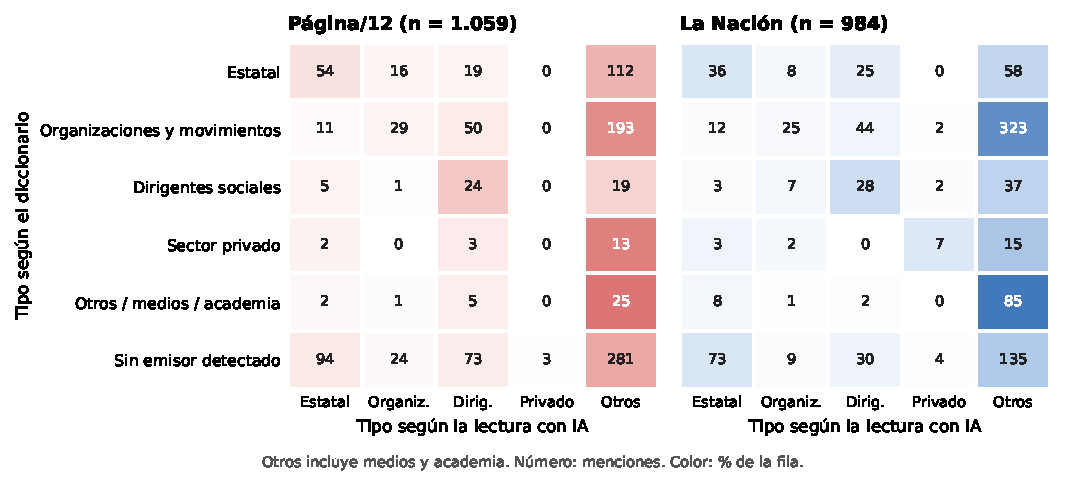
\includegraphics[width=\linewidth]{fig/fig_confusion_emisor.pdf}\\[6pt]
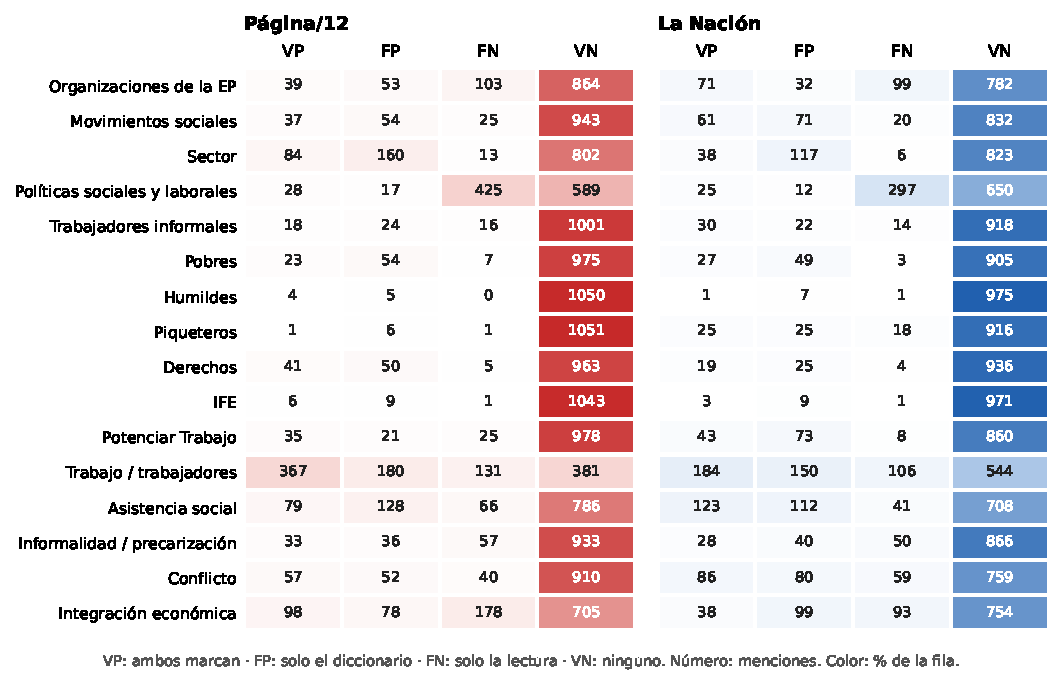
\includegraphics[width=\linewidth]{fig/fig_confusion_marcos.pdf}
\caption{Matrices de confusión entre el diccionario y la lectura con IA, por diario. Arriba, tipo de emisor principal; abajo, cada marco de forma binaria. La lectura es una referencia y falta validarla con el equipo.}
\label{fig:confusion}
\end{figure}


\paragraph{Revisión de casos atribuidos a ANSES.} La primera lectura con IA había registrado a la ANSES entre los emisores más citados. Se revisaron una por una las 32 menciones cuyo fragmento nombra al organismo. Trece correspondían en realidad a la voz del diario, una a Amado Boudou, dos a una columna firmada en nombre de las organizaciones de la \EP{} y dieciséis a una cita textual de la ANSES en la que el término aparece solo dentro del nombre del registro. Veinticinco de las 32 eran menciones \enquote{solo nombre}. Este caso muestra el principal riesgo de la lectura automatizada - atribuir el término a quien aparece cerca y no a quien lo pronuncia - y la necesidad de revisar muestras a mano. En la lectura mención por mención, el tipo de emisor coincide con esta revisión manual en 30 de las 32 menciones y la marca de \enquote{solo nombre} en 31.

\subsection{Problemas y desafíos técnicos}

\begin{table}[h]
\centering\small
\caption{Principales desafíos y cómo se abordaron.}
\label{tab:desafios}
\begin{tabularx}{\linewidth}{>{\raggedright}p{3.3cm} >{\raggedright}X >{\raggedright\arraybackslash}X}
\toprule
\textbf{Desafío} & \textbf{Qué ocurrió} & \textbf{Cómo se abordó} \\
\midrule
Buscadores dinámicos & Los resultados se cargan con JavaScript; los pedidos HTTP simples no devuelven nada. & Automatización de navegador con Playwright. \\
Búsqueda imprecisa en \pdoce & Sin comillas, 82.690 resultados; con filtro de fecha, error 404. & Frase exacta entre comillas y filtro de fecha en Python. \\
Ruido en los enlaces de \lanac & La recolección por desplazamiento traía unos 13.000 enlaces ajenos a la búsqueda. & Filtrado posterior por contenido: solo quedan notas que contienen el término. \\
Muro de pago de \lanac & El muro medido bloquea la lectura tras pocas notas. & Wayback Machine y, luego, la suscripción institucional autorizada. \\
Inicio de sesión bloqueado & Google no permite iniciar sesión desde ventanas automatizadas. & Inicio de sesión manual y conexión de Playwright a esa sesión. \\
Procesos largos & Colab interrumpe sesiones largas; cada nota demora varios segundos. & Puntos de control en Drive para retomar sin repetir pedidos. \\
Límite de Excel & 8 notas largas se truncaron en 32.767 caracteres, el máximo de una celda. & Documentado; se propone exportar a CSV o Parquet. \\
Diccionario insuficiente & No ve la voz del diario y confunde nombre con concepto. & Lectura completa asistida por IA, comparación sistemática y corrección del marco trabajo. \\
\bottomrule
\end{tabularx}
\end{table}

Otra dificultad fue el entorno de trabajo. Al comenzar, mi experiencia con la terminal, los entornos virtuales y las rutas de archivos era limitada, lo que demandó tiempo en las primeras semanas. Reorganizar el procesamiento en cuadernos de Colab encadenados, que leen y escriben en una misma carpeta de Drive, simplificó la ejecución y la hizo reproducible para el resto del equipo.

\subsection{Limitaciones}
\label{sec:limitaciones}

\begin{itemize}
  \item \textbf{Cobertura de \pdoce.} El corpus de \pdoce{} contiene exactamente 600 notas, mientras que la API informó 2.330 resultados para la búsqueda (sin filtro de fecha). Además, no hay notas de ese diario entre septiembre y noviembre de 2019 ni en el segundo trimestre de 2020, el primero de 2021 y el primero de 2023 (Figura~\ref{fig:trimestre}). La cifra redonda y los huecos sugieren un corte en la paginación de la recolección, que debe verificarse. Mientras tanto, las comparaciones entre diarios y en el tiempo deben leerse con cautela.
  \item \textbf{Fechas de \pdoce.} Cinco notas figuran con fecha 10 de agosto de 2022, aunque por su título y contenido parecen ser de 2019. Se detectaron durante la lectura y no se corrigieron, por lo que pueden afectar levemente las series por año y por trimestre. No se revisaron sistemáticamente las fechas del resto del corpus.
  \item \textbf{Textos incompletos.} 30 notas de \pdoce{} no tienen texto y 8 notas largas están truncadas por el límite de celda de Excel.
  \item \textbf{Diccionario.} La codificación por patrones depende de una ventana de 300 caracteres y de nombres explícitos; no reconoce la voz del medio ni distingue con seguridad a quien habla de quien es mencionado.
  \item \textbf{Lectura con IA.} Fue realizada por 45 lectores automáticos en paralelo y presenta variación de criterio entre lotes. Sus resultados no fueron todavía validados por codificación humana del equipo.
  \item \textbf{Alcance.} Dos medios no representan al conjunto de la prensa nacional; las conclusiones se refieren a estos dos diarios.
\end{itemize}

% =====================================================================
\section{Ajustes y diferencias respecto de lo previsto}
% =====================================================================

La Tabla~\ref{tab:objetivos} resume el grado de cumplimiento de cada objetivo específico.

\begin{table}[h]
\centering\small
\caption{Grado de cumplimiento de los objetivos del Plan de Trabajo.}
\label{tab:objetivos}
\begin{tabularx}{\linewidth}{c >{\raggedright}p{4.4cm} >{\raggedright}p{2.4cm} >{\raggedright\arraybackslash}X}
\toprule
\textbf{\#} & \textbf{Objetivo} & \textbf{Estado} & \textbf{Qué se hizo} \\
\midrule
1 & Base de notas de ambos diarios & Cumplido, con limitaciones & 1.245 notas con metadatos y texto completo; cobertura de \pdoce{} a verificar. \\
2 & Análisis exploratorio & Cumplido & Serie temporal por diario, secciones, autores y menciones por nota. \\
3 & Identificar emisores & Cumplido, con otro método & Codificación por libro de códigos (diccionario y lectura completa) en lugar de reconocimiento de entidades genérico. \\
4 & Redes de co-ocurrencia & Parcial & Tablas cruzadas emisor $\times$ marco, generales y por diario; no se construyeron los grafos de red. \\
5 & Clasificar menciones por marco & Cumplido, con otro método & 16 marcos del libro de códigos del equipo, en lugar del diccionario inductivo de 9 marcos previsto. \\
6 & \textit{Word embeddings} y sentimiento & No realizado & Ver justificación. \\
7 & Visualizaciones y documentación & Cumplido & Scripts y cuadernos encadenados, gráficos, presentación en las Jornadas (04/11/2026) y este informe. \\
\bottomrule
\end{tabularx}
\end{table}

\paragraph{Cambio de método en los objetivos 3 y 5.} Durante el proyecto, el equipo de ciencias sociales elaboró un libro de códigos detallado, con cinco tipos de emisor y dieciséis marcos. Tomarlo como base hizo que los resultados fueran interpretables por el equipo y comparables con su codificación manual. Además, el reconocimiento de entidades genérico producía mucho ruido sobre este corpus: en una primera prueba, el \enquote{actor} más frecuente que devolvía era el propio término \enquote{Economía Popular} escrito con mayúsculas (301 casos). Por eso se decidió cambiar el método.

\paragraph{Objetivos 4 y 6.} La construcción del corpus demandó más tiempo del previsto, en particular por el muro de pago de \lanac{}, que obligó a probar dos estrategias de recolección sucesivas. Con el tiempo restante se priorizó validar la codificación de emisores y marcos, que responde directamente a la pregunta de investigación, por sobre los análisis complementarios. El Plan de Trabajo ya preveía que el objetivo 6 quedaba sujeto al avance del corpus. Las tablas emisor $\times$ marco del objetivo 4 están calculadas; resta representarlas como redes.

\paragraph{Cambios que no estaban en el plan.} Se incorporaron dos actividades no previstas: la comparación sistemática entre dos vías de codificación, que permitió detectar y corregir sesgos del diccionario, y la identificación de las menciones que son solo parte de un nombre propio, que abrió una discusión conceptual con el equipo.

\paragraph{Plazos y dedicación.} El trabajo se extendió entre el 3 de agosto y el 13 de noviembre de 2026, de acuerdo con lo previsto.

\begin{table}[h]
\centering\small
\caption{Tiempo invertido por etapa.}
\begin{tabular}{llr}
\toprule
\textbf{Período} & \textbf{Etapa} & \textbf{Horas} \\
\midrule
Agosto & Marco conceptual, plan de trabajo y orientación técnica & 12 \\
Septiembre & Recolección de \pdoce{} y primera etapa de \lanac{} & 24 \\
Septiembre--octubre & Análisis exploratorio e informe de avance & 12 \\
Octubre & \lanac{} con suscripción; menciones; codificación & 24 \\
Octubre--noviembre & Validación y corrección del diccionario & 12 \\
Noviembre & Presentación en las Jornadas e informe final & 12 \\
\midrule
\textbf{Total} & & \textbf{96} \\
\bottomrule
\end{tabular}
\end{table}

% =====================================================================
\section{Aprendizajes y vínculo con la Ciencia de Datos}
% =====================================================================

\subsection{Competencias técnicas}

\begin{itemize}
  \item \textbf{Recolección de datos de la web.} Aprendí a automatizar un navegador con Playwright, a inspeccionar el tráfico de red para encontrar las fuentes de datos internas de un sitio y a preferir estructuras de datos estables por sobre selectores visuales. También aprendí a respetar las condiciones de acceso, a resolver el muro de pago por vías institucionales y a documentar las limitaciones.
  \item \textbf{Procesos largos y reproducibles.} Diseñé un procesamiento por etapas con puntos de control, deduplicación por clave y archivos intermedios, de modo que cualquier etapa pueda reejecutarse y que otra persona del equipo pueda reproducir el trabajo.
  \item \textbf{Depuración sistemática.} Varios problemas, como los parámetros de la API de \pdoce{}, solo pudieron aislarse cambiando una cosa por vez.
  \item \textbf{Procesamiento de texto.} Trabajé con expresiones regulares tolerantes a variantes, diccionarios auditables y métricas de cobertura y precisión para evaluarlos.
  \item \textbf{Uso crítico de modelos de lenguaje.} Un modelo de lenguaje puede leer y codificar un corpus completo siguiendo un libro de códigos, pero su salida necesita validación: el caso de la ANSES mostró que puede atribuir el término a quien aparece cerca y no a quien lo pronuncia.
\end{itemize}

\subsection{Aprendizajes metodológicos e interdisciplinarios}

\begin{itemize}
  \item \textbf{Categorías del equipo.} El libro de códigos del equipo de ciencias sociales fue lo que le dio sentido al código. Sin él, el reconocimiento de entidades producía listas de nombres sin interpretación posible.
  \item \textbf{Lectura de las notas.} Que un tercio de las menciones fueran solo un nombre se vio al leer las notas, y eso abrió una discusión conceptual sobre qué cuenta como uso del término.
  \item \textbf{Decisiones técnicas.} El tamaño de la ventana de contexto, la forma de contar las repeticiones o el tratamiento de los nombres de organizaciones cambian los resultados. Por eso deben acordarse con el equipo y documentarse.
  \item \textbf{Comparación de métodos.} Contrastar el diccionario con la lectura completa sirvió para ver dónde y por qué difieren, y para corregir el diccionario.
\end{itemize}

\subsection{Vínculo con la Ciencia de Datos y con la trayectoria profesional}

En la práctica trabajé en todas las etapas de un proyecto de datos: definición del problema con el equipo usuario, obtención de los datos, limpieza, modelado, validación y comunicación de resultados a un público no técnico, incluida la presentación en las Primeras Jornadas Interdisciplinarias de Ciencia de Datos e IA. Usé contenidos de distintas materias de la carrera - programación, procesamiento de texto, visualización y análisis de datos - y, en particular, los de Gobernanza de Datos y Equidad en Aprendizaje Automático, en relación con el acceso responsable a las fuentes, el tratamiento de material protegido por derecho de autor y los sesgos de los métodos automáticos.

En relación con mi trayectoria profesional como analista de datos en investigación en salud, la práctica me dejó dos aprendizajes: la importancia de que un procesamiento de datos sea reproducible y auditable por personas de otras disciplinas, y la necesidad de validar cualquier clasificación automática contra una lectura experta antes de usar sus resultados. Al mismo tiempo, me permitió trabajar por primera vez con datos textuales no estructurados y con preguntas de las ciencias sociales, lo que amplió el tipo de problemas que puedo abordar desde la Ciencia de Datos.

% =====================================================================
\section*{Materiales adjuntos}
\addcontentsline{toc}{section}{Materiales adjuntos}
% =====================================================================

Por tratarse de material protegido por derecho de autor, el texto completo de las notas se conserva para uso interno del equipo y no se redistribuye; se entregan el código y los datos derivados.

\begin{table}[h]
\centering\small
\footnotesize\begin{tabularx}{\linewidth}{>{\ttfamily\raggedright}p{7.4cm} X}
\toprule
\normalfont\textbf{Archivo} & \textbf{Contenido} \\
\midrule
src/01\_scraper/ & Recolección de \pdoce{} y \lanac{} con puntos de control. \\
src/02\_extraer\_fragmentos.py & Detección de menciones y recorte de contexto. \\
src/03\_codificacion\_diccionario.py & Codificación por diccionario (con la corrección del marco trabajo) y tablas emisor $\times$ marco. \\
src/04\_lectura\_llm/ & Instrucciones, lotes y unión de la lectura mención por mención. \\
src/05\_comparacion\_metodos.py & Matrices de confusión entre las dos vías. \\
fragmentos\_codificados.xlsx & Una fila por mención con emisores y marcos detectados. \\
tabla\_emisores\_marcos.xlsx & Cruces tipo, subtipo y emisor $\times$ marco. \\
fragmentos\_codificados\_revision\_anses.xlsx & Revisión manual de las 32 menciones vinculadas a ANSES. \\
corpus\_final\_codificado\_sin\_nota.xlsx & Las 2.043 menciones con ambas codificaciones, sin el texto de las notas. \\
comparacion\_metodos.xlsx & Métricas por marco, tipo y diario, y desacuerdos más frecuentes. \\
\bottomrule
\end{tabularx}
\end{table}

\section*{Referencias}
\addcontentsline{toc}{section}{Referencias}
\begin{itemize}[leftmargin=1.2em, label={}]
  \item \label{benford2000}Benford, R. D. y Snow, D. A. (2000). Framing processes and social movements: An overview and assessment. \textit{Annual Review of Sociology}, 26, 611--639.
  \item Microsoft (s.\,f.). \textit{Playwright for Python}. \url{https://playwright.dev/python/}
  \item The pandas development team (s.\,f.). \textit{pandas}. \url{https://pandas.pydata.org/}
\end{itemize}

\end{document}
